\section{Macchine termodinamiche}
Con il termine di \textbf{macchina termodinamica} si intende un sistema composto da un opportuna
combinazione di sottosistemi elementari (serbatoio di calore, serbatoio di lavoro e macchina
ciclica) che ha come funzione o la conversione termodinamica di energia termica in lavoro
(\textbf{macchina termodinamica motrice}) o il trasferimento di energia termica da uno o più serbatoi
di calore a temperatura inferiore a uno o più serbatoi di calore a temperatura superiore
(\textbf{macchina termodinamica operatrice}). \newline
\newline
Per \textbf{serbatoio di calore} si intende un sistema termodinamico che scambia \textbf{solo calore} con l'esterno senza alterare il suo stato termodinamico (cioè la temperatura e la pressione del serbatoio rimangono costanti, il suo stato non cambia); gli scambi avvvengono con trasformazioni quasi-statiche (\textbf{internamente reversibili}). Questa definizione di serbatoio è sinonimo di un sistema \textbf{a massa infinita}.\newline
\newline
Per \textbf{serbatoio di lavoro} si intende un sistema termodinamico che scambia \textbf{solo lavoro} con l'esterno senza alterare il suo stato termodinamico; gli scambi avvengono con trasformazioni quasi-statiche (\textbf{internamente reversibili}).
\subsection{macchina motrice con sorgenti a temperatura cosante}
\begin{center}
    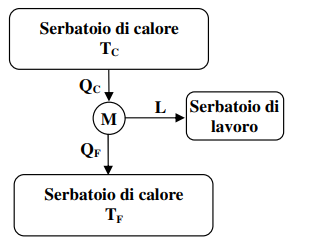
\includegraphics[height=5cm]{../NOTE SUGLI ESERCIZI/img4.PNG}
\end{center}
Vediamo la macchina motrice da un punto di vista analitico.\newline
Dalle equazioni di bilancio otteniamo:
\[
    \begin{cases}
        \Delta U_Z = 0\\ \Delta S_Z = S_{irr}
    \end{cases} \;\;\;\;\;\;\;\;\;\;\;\;\;\;\; \begin{cases}
        \Delta U_C + \Delta U_F + \Delta U_{SL} + \Delta U_M = 0 \\
        \Delta S_C + \Delta S_F + \Delta S_{SL} + \Delta S_M = S_{irr}
    \end{cases}
\]
Osservando i singoli sottosistemi otteniamo:
\[
    \begin{cases}
        \Delta U_C = Q_C^\leftarrow \\ \Delta S_C = \frac{Q_C^\leftarrow }{T_C}
    \end{cases} \;\;\;\;\; \begin{cases}
        \Delta U_F = Q_F^\leftarrow \\ \Delta S_F = \frac{Q_F^\leftarrow}{T_F}
    \end{cases} \;\;\;\;\; \begin{cases}
        \Delta U_{SL} = - L_{SL}^\rightarrow \\ \Delta S_{SL} = 0
    \end{cases} \;\;\;\;\; \begin{cases}
        \Delta U_M = 0\\ \Delta S_M = 0
    \end{cases}
\]
Dai bilanci energetico ed entropico della macchina termodinamica motrice illustrata in figura
e che è caratterizzata da operare con serbatoi di calore a temperatura costante $T_S$ e $T_F$, si
ottiene: 
\[
    \begin{cases}
        Q_C^\leftarrow  + Q_F^\leftarrow  - L_{SL}^\rightarrow = 0\\
        \frac{Q_C^\leftarrow}{T_C} + \frac{Q_C^\leftarrow}{T_F} = S_{irr}
    \end{cases}\;\;\;\;\;\longrightarrow\;\;\;\;\;\begin{cases}
        -Q_C + L + Q_F = 0\\
        - \frac{Q_C}{T_C} + \frac{Q_F}{T_F} = S_{irr}
    \end{cases}
\]
\ \newline
L’analisi termodinamica di una macchina termodinamica motrice richiede spesso di separare
l’analisi della macchina ideale (reversibile) che consente di massimizzare il lavoro prodotto
da quella reale (irreversibile). \newline
Nel caso di macchina termodinamica motrice \textbf{ideale}, o reversibile, si ottiene: 
\[
    L_{rev} = Q_C \left(1- \frac{T_F}{T_C}\right)
\]
\[
    \eta_{rev} = 1- \frac{T_F}{T_C}
\]
\ \newline
Nel caso di macchina termodinamica motrice \textbf{reale}, o irreversibile, si ottiene:
\[
    L  = Q_C \left(1- \frac{T_F}{T_C}\right) - T_FS_{irr}
\]
\[
    \eta = \frac{L}{Q_C} = 1-\frac{T_F}{T_C} - \frac{T_F S_{irr}}{Q_C}
\]
\ \newline
Questi concetti consentono di introdurre il concetto di \textbf{lavoro perso} (o dissipato):
\[
    L_P = L_{rev} - L \;\;\;\;\;\;\;\;\;\;\;\;\;\;\;L_{P} = T_FS_{irr}
\]
che rappresenta l’energia che il sistema termodinamico reale non è in grado di convertire in
lavoro utile a causa di una non-idealità intrinseca del processo di conversione analizzato.
\subsection{macchina operatrice con sorgenti a temperatura costante}
\begin{center}
    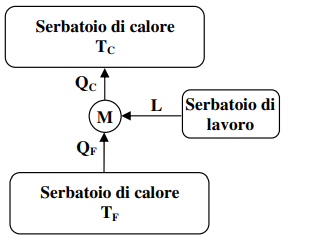
\includegraphics[height=5cm]{../NOTE SUGLI ESERCIZI/img5.PNG}
\end{center}
Vediamo la macchina operatrice da un punto di vista analitico.\newline
Dalle equazioni di bilancio otteniamo:
\[
    \begin{cases}
        \Delta U_Z = 0\\ \Delta S_Z = S_{irr}
    \end{cases} \;\;\;\;\;\;\;\;\;\;\;\;\;\;\; \begin{cases}
        \Delta U_C + \Delta U_F + \Delta U_{SL} + \Delta U_M = 0 \\
        \Delta S_C + \Delta S_F + \Delta S_{SL} + \Delta S_M = S_{irr}
    \end{cases}
\]
Osservando i singoli sottosistemi otteniamo:
\[
    \begin{cases}
        \Delta U_C = Q_C^\leftarrow \\ \Delta S_C = \frac{Q_C^\leftarrow }{T_C}
    \end{cases} \;\;\;\;\; \begin{cases}
        \Delta U_F = Q_F^\leftarrow \\ \Delta S_F = \frac{Q_F^\leftarrow}{T_F}
    \end{cases} \;\;\;\;\; \begin{cases}
        \Delta U_{SL} = - L_{SL}^\rightarrow \\ \Delta S_{SL} = 0
    \end{cases} \;\;\;\;\; \begin{cases}
        \Delta U_M = 0\\ \Delta S_M = 0
    \end{cases}
\]
Dai bilanci energetico ed entropico della macchina termodinamica operatrice illustrata in
figura e che è caratterizzata da operare con serbatoi di calore a temperatura costante $T_C$ e $T_F$ si
ottiene:
\[
    \begin{cases}
        Q_C^\leftarrow  + Q_F^\leftarrow  - L_{SL}^\rightarrow  = 0\\
        \frac{Q_C^\leftarrow}{T_C} + \frac{Q_F^\leftarrow}{T_F} = S_{irr}
    \end{cases} \;\;\;\;\;\longrightarrow\;\;\;\;\;\begin{cases}
        +Q_C - L - Q_F = 0\\
        + \frac{Q_C}{T_C} - \frac{Q_F}{T_F} = S_{irr}
    \end{cases}
\]
Rispetto alla macchina motrice è differente l’equazione di bilancio entropico in quanto
cambiano i segni dei contributi associati ai serbatoi di calore e di lavoro.\newline
\newline
Anche in questo caso si separa l’analisi della macchina termodinamica ideale (reversibile) per
la quale viene minimizzato il lavoro necessario per realizzare il processo, rispetto alla
macchina termodinamica operatrice reale (o irreversibile). \newline
Nel caso di macchina termodinamica operatrice \textbf{ideale}, o reversibile, si ottengono le due
relazioni: 
\[
    L_{rev,F} = Q_F\left(\frac{T_C}{T_F}-1\right) \;\;\;\;\;\;\;\;\;\;\;\;\;\;\; L_{rev,PC} = Q-C \left(1- \frac{T_F}{T_C}\right)
\]
che si differenziano per il fatto di consentire la valutazione del lavoro assorbito in funzione
del calore prelevato dalla sorgente inferiore (analisi tipica della macchina \textbf{frigorifera}) o del
lavoro assorbito in funzione del calore ceduto alla sorgente di lavoro (analisi tipica della
\textbf{pompa di calore}).
\newline
\newline
Nel caso di macchina termodinamica operatrice \textbf{reale}, o irreversibile, si ottengono: 
\[
    L = Q_F\left(\frac{T_C}{T_F}-1\right) + T_C S_{irr} \;\;\;\;\;\;\;\;\;\;\;\;\;\;\; L = Q_C \left(1- \frac{T_F}{T_C}\right) + T_F S_{irr}
\]
Il lavoro assorbito è in questo caso maggiore rispetto a quello assorbito nel caso ideale. \newline
\newline
Come parametro di merito si introduce, per le macchine termodinamiche operatrici
l’efficienza $\epsilon$ (anche detto COP). \newline
\newline
Nel caso di funzionamento come macchina \textbf{frigorifera} si ha: 
\[
    \epsilon_{f,rev} = \frac{T_F}{T_C-T_F} \;\;\;\;\;\;\;\;\;\;\;\;\;\;\; \epsilon_{f} = \frac{Q_F}{L} = \frac{T_F}{T_C-T_F + \frac{T_CT_FS_{irr}}{Q_F}}
\]
Nel caso di funzionamento come \textbf{pompa di calore} si ha:
\[
    \epsilon_{PC, rev} = \frac{T_C}{T_C-T_F} \;\;\;\;\;\;\;\;\;\;\;\;\;\;\; \epsilon_{PC} = \frac{Q_C}{L} = \frac{T_C}{T_C-T_F + \frac{T_CT_FS_{irr}}{Q_C}}
\]
\ \newline
Legame fra efficienza della macchina frigorifera e della pompa di calore:
\[
    \epsilon_P = \frac{Q_C}{L} = \frac{Q_F + L}{L} = \epsilon_F +1
\]
\subsection{Macchina motrice con serbatoio caldo a massa finita}
Vedi teoria per un esempio.
\subsection{Rendimento di secondo principio}
Il rendimento di una macchina termodinamica motrice e l’efficienza (o il COP) di una
macchina termodinamica operatrice rappresentano il cosiddetto \textbf{rendimento di primo
principio} che è un indice della capacità del processo di conversione dell’energia di soddisfare
gli obiettivi a fronte di una certa spesa energetica. \newline
\newline
Viene anche introdotto il concetto di \textbf{rendimento di secondo principio} che rappresenta la
capacità di un processo reale di avvicinarsi alle prestazioni del processo ideale (che nel caso
termodinamico è il processo reversibile per il quale non si ha produzione di entropia per
irreversibilità). Per la macchina termodinamica motrice e per la macchina termodinamica
operatrice (frigorifera o pompa di calore) si ha: 
\[
    \eta_{II} = \frac{L}{L_{rev}} \;\;\;\;\;\;\;\;\;\;\;\;\;\;\; \eta_{II} = \left(\frac{\eta}{\eta_{rev}}\right)_{Tc, Qc, Tf}
\]
\[
    \eta_{II} = \frac{L_{rev}}{L} \;\;\;\;\;\;\;\;\;\;\;\;\;\;\; \eta_{II} = \left(\frac{\epsilon}{\epsilon_{rev}}\right)_{Tc,Tf,Qf}
\]
\ \newline
\textbf{oss.} i risultati che sono stati ottenuti valgono solo per macchine termodinamiche con
sorgenti a temperatura costante. 